\section{Power supply and electrical interfacing}
The different onboard devices need different power supplies: in particular, the coil and transistor need 12V to operate in series, the mouse interface, Hall effect sensor and the Stellaris board need a 5V supply (the Stellaris microcontroller is fed by the onboard 3.3V regulator, which has 5V input used also for USB communication), while all the digital logic and the flash memory need 3.3V. Also, the ADC input amplifier needs a negative voltage source to be able to operate correctly when the SS495 output is near to 0V.

The main power source is a 12V, 1A transformer from an old device. This provides lots of power, although with quite a high noise level as it comes from a switched PSU. Thus, first of all a big electrolytic capacitor ($1000\mu F$) in parallel with a smaller (100nF), ceramic one, filter the input voltage leaving a clean 12V voltage rail. To this rail are connected two TO-220 linear regulators, an LM317 programmed to give 5V as output and a fixed-voltage LM1086 regulator providing the 3.3V rail. The 5V line, feeding the Hall effect sensor, is further cleaned with another $1000\mu F$ capacitor as the latter is very sensible to input voltage fluctuations. For the 3.3V line, instead, only a $2.2\mu F$ capacitor is used as sensibility to noise is far less.

Power dissipation on the 3.3V line is quite high, as this has been attached to the 12V rail and not to the 5V one in order to avoid voltage drops on the latter, leaving clean sensor readings. With about 9V of voltage drop on the regulator, the power consumption of the regulator is about 0.75W (both the flash memory and the CPLD consume about 35mA of current). Without a heat dissipator, this leads the LM1086's package to have a quite high temperature after some minutes of use, but it seems that it is tolerable anyway. A little aluminum pad has been added in order to solve this problem.

In order to feed the ADC's operational amplifier with a negative voltage, an LM555 IC has been configured as an oscillator, and its output connected to a charge pump. This creates a negative charge on the output capacitor, which is quite big in order to provide a stable power rail also from this unstable supply.

\begin{figure}[htbp]
\centering
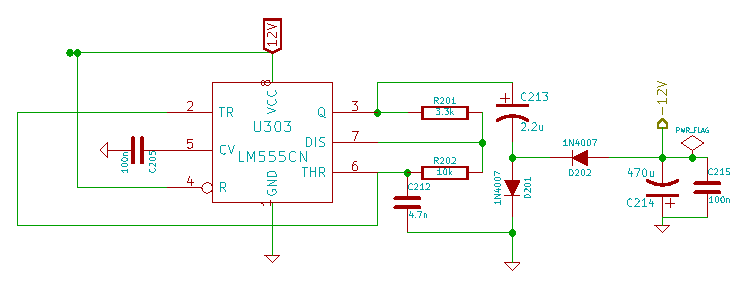
\includegraphics[width=4in]{Graphics/Supply}
\caption{Schematics for the negative supply rail}
\end{figure}


